\chapter{TỔNG QUAN}
\ifpdf
    \graphicspath{{Chapter2/Chapter2Figs/PNG/}{Chapter2/Chapter2Figs/PDF/}{Chapter2/Chapter2Figs/}}
\else
    \graphicspath{{Chapter2/Chapter2Figs/EPS/}{Chapter2/Chapter2Figs/}}
\fi

\section{Giới thiệu bài toán Topic Detection and Tracking}
Topic Detection and Tracking (TDT) là một dự án được khởi xướng từ năm 1996, với nhiệm vụ nghiên cứu, phát triển công nghệ cho việc lưu trữ, tổ chức, tìm kiếm dữ liệu từ các nguồn \textit{tin tức}. TDT được chia làm 5 tác vụ chính: Story segmentation, Topic tracking, Topic detection, \textit{First story detection} và Link detection.

\section{Bài toán First Story Detection}
Bài toán First Story Detection (FSD), hay còn gọi là New Event Detection (NED), được đặt ra với mục tiêu phát hiện các tin tức, bài viết đầu tiên trên báo chí về các sự kiện vừa xảy ra, chưa từng được báo cáo trước đó. Một hệ thống có khả năng phát hiện các first story có thể cung cấp thông tin có giá trị cho các nhà phân tích, các biên tập viên báo chí một cách nhanh chóng, kịp thời.

Ngoài nguồn dữ liệu từ báo đài chính thống, các bài viết từ mạng xã hội cũng là một nguồn tin có tiềm năng rất lớn. 
%34.7tr ng FB 2016, 

	\begin{definition}
		Event (sự kiện) là một sự việc bất kì, xảy ra tại một địa điểm cụ thể, vào thời điểm xác định.
	\end{definition}
	\begin{definition}
		Story là một bài viết về một sự kiện nhất định. Có ít nhất 2 câu trần thuật độc lập với nhau.
	\end{definition}

%To aid the LDC’s annotation of story boundaries, the community agreed that a story is “a topically cohesive segment of news that includes two or more declarative independent clauses about a single event.” While the definition doesn’t address stories that discuss multiple events, which happens frequently in the TDT corpora, the definition enabled the LDC to tag the data with story boundaries with adequate reliability.

%In the TDT pilot study, the notion of a topic was limited to be an “event”, meaning something that happens at some specific time and place along with all necessary preconditions and unavoidable consequences. Later, in the second year, the definition of a topic was broadened to include, in addition to the triggering event, other events and activities that are directly related to it. This definition has persisted for the ensuing years. Formally, the TDT definition of a topic is “a seminal event or activity, along with all directly related events and activities.” A story is considered “on topic” when it discusses events and activities that are directly connected to that topic’s seminal event. Therefore, for example, a story on the search for survivors of an airplane crash, or on the funeral of the crash victims, will be considered a story on the crash event. Obviously there must be limits to this inclusiveness. (For example, stories on FAA repair directives that derive from a crash investigation would not be considered stories on the crash event.) Since definition of a topic’s extension to related events is not readily agreed upon, the LDC has created topic annotation guidelines to improve agreement and consistency of topic labelling. [5]


%\section{Biểu diễn dữ liệu bằng Vector space model và tf-idf}

\section{Tiếp cận bằng phương pháp gom cụm}
%đoạn này trình bày ý tưởng giải FSD? tìm document tương đồng nhất, khi vượt ngưỡng ==> first story
%ngoài ra còn cách gom cụm truyền thống?
\subsection{Giới thiệu một số độ đo khoảng cách/sự tương đồng} \label{distances}
	Một thành phần tất yếu của tiếp cận gom cụm là tiêu chí, độ đo được sử dụng để định lượng sự tương đồng giữa các document. Dưới đây là một số độ đo phổ biến.
	\subsubsection*{Euclidean Distance}
	Euclidean Distance là độ đo khoảng cách tiêu chuẩn trong các vấn đề liên quan đến hình học, và cũng thường được sử dụng trong các bài toán gom cụm. 
	\begin{equation}
		D_{Euclidean}(\vec{x}, \vec{y}) = \sqrt{\sum_{i=1}^n (x_i-y_i)^2}
	\end{equation}
	với n là số chiều của vector biểu diễn document, $x_i$ và $y_i$ lần lượt là giá trị tọa độ thứ i của document x và y\\

	\subsubsection*{Cosine Similarity}
	Cosine Similarity phản ánh góc chênh lệch giữa 2 vector, mà không cân nhắc đến độ lớn của vector. Độ đo này được áp dụng rộng rãi đối với dữ liệu văn bản.
	\begin{equation}
		D_{Cosine}(\vec{x}, \vec{y}) = \frac {\vec{x} \cdot \vec{y}}{||\vec{x}|| \cdot ||\vec{y}||} = \frac{\sum_{i=1}^{n}x_iy_i}{\sqrt{\sum_{i=1}^{n}x_i^2} \sqrt{\sum_{i=1}^{n}y_i^2}}	
	\end{equation}
	với  $x_i$ và $y_i$ lần lượt là giá trị tọa độ thứ i của document x và y
	
\subsection{Thuật toán tìm láng giềng gần nhất (Nearest Neighbor Search)}
	\subsubsection{Ý tưởng}
	%sửa lại chỉ nói về NNS thôi chứ không nói ý tưởng giải FSD?
	Hướng tiếp cận truyền thống của bài toán FSD là sử dụng phương pháp tìm láng giềng gần nhất. Theo trực quan ta có thể thấy nếu một bài viết có nội dung tương tự nhiều với những bài có sẵn, thì khả năng nó là một first story rất thấp. Ngược lại, khi nội dung của một bài viết mới lạ, khác hẳn những bài viết trước đây, thì có thể xem đó là một first story. 
	
	Thuật toán tìm láng giềng gần nhất hoạt động như sau: Mỗi document mới sẽ được so sánh với tất cả các document hiện có trong hệ thống và tìm ra một document tương đồng nhất. Nếu độ tương đồng của chúng thấp hơn một ngưỡng cho trước, thì document mới này sẽ được xem như một first story.\\
	
	\subsubsection{Minh họa thuật toán}
	Giả sử ta có dữ liệu như hình vẽ. Đường tròn thể hiện ngưỡng khoảng cách để một document được xem là first story hay không, chọn ngưỡng giá trị 0.8. Ta có sẵn 4 document và 1 document mới vào hệ thống như sau:\\
	doc1 = (3,4,1,2)\\
	doc2 = (1,1,5,6)\\
	doc3 = (1,2,4,4)\\
	doc4 = (3,5,1,1)\\
	newDoc = (2,1,4,5)\\
	\begin{table}[H]
		\centering
		\begin{tabular}{p{1.5cm}|p{1.5cm}|p{1.5cm}|p{1.5cm}|p{1.5cm}|p{1.5cm}}
			\hline
			& doc1 & doc2 & doc3 & doc4 & \textbf{newDoc} \\
			\hline 
			doc1 & 1 & 0.55202 & 0.6903 	& 0.973729 & 0.646058 \\
			doc2 &   & 1 		& 0.973479 	& 0.398962 & 0.984525 \\
			doc3 &   &   		& 1			& 0.575396 & 0.969572 \\
			doc4 &   &  		&  			& 1 	& 0.491473 \\
			newDoc &   &  		&  			&   	& 1 \\
			\hline
		\end{tabular}
		\caption{Độ tương đồng cosine giữa các document} \label{tab:table_1_1}
	
	\end{table}
	Ta có thể thấy document tương tự nhất của newDoc là doc2 (0.984525), lớn hơn ngưỡng cho trước (0.8), do đó newDoc không phải là một first story.

	\begin{figure}[H]
		\begin{center}
			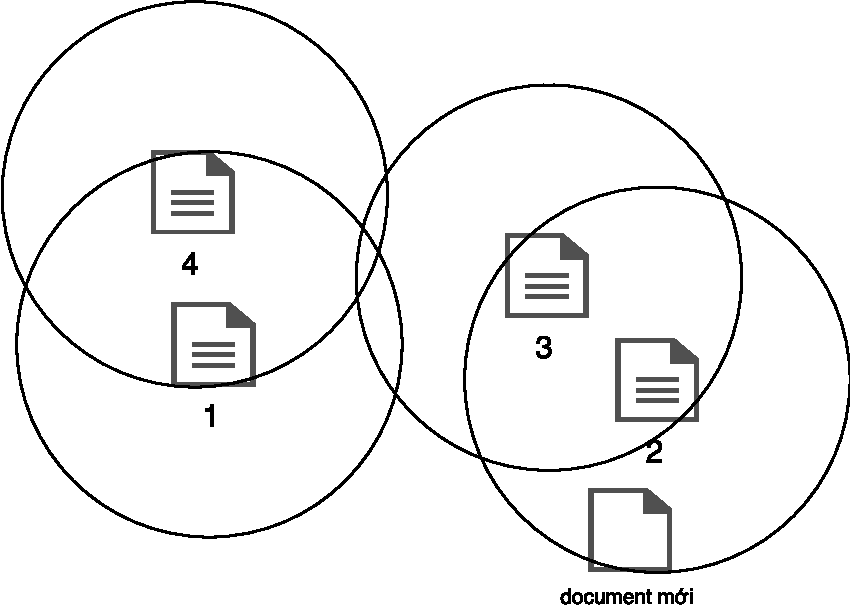
\includegraphics[]{NNS.pdf}
			\caption{...}
		\end{center}
	\end{figure}
	
	\subsubsection{Mã giả}
	\begin{algorithm}[H]
		\caption{First Story Detection dựa trên Nearest neighbor search}
		\begin{algorithmic}[1]
			\REQUIRE luồng bài viết từ Twitter, giá trị ngưỡng t
			\ENSURE những document được cho là first story
			\ForEach{document $d$ trong toàn bộ dữ liệu}
			\State $S(d) \leftarrow \emptyset$
			\ForEach{term $t$ trong document $d$}
			\ForEach{document $d'$ trong $index[t]$}
			\State cập nhật khoảng cách $distance(d,d')$
			\State $S(d) \leftarrow S(d) \cup d'$
			\ENDFOR 
			\State $index[t] \leftarrow index[t] \cup d$ (thêm document $d$ vào index của term t)
			\ENDFOR
			\STATE novelty score của d: $dis_{min}(d) \leftarrow 1$
			
			\ForEach{document $d'$ trong S(d)}
			\IF{$distance(d,d') < dis_{min}(d)$}
			\STATE $dis_{min}(d) \leftarrow distance(d,d')$
			\ENDIF
			\ENDFOR
			\IF{$dis_{min}(d) >= t$}
			\STATE d là một first story
			\ENDIF
			\ENDFOR	
			
		\end{algorithmic}
	\end{algorithm}
	Chú thích thuật toán:
	\begin{itemize}
		\item $t$: ngưỡng để xét một document có phải là first story hay không
		\item $S(d)$: tập document có ít nhất 1 term chung với $d$
		\item $distance(d,d')$: khoảng cách giữa document $d$ và $d'$, có thể sử dụng các độ đo ở mục \ref{distances}
		\item $index(t)$: danh sách cách document có chứa term $t$
		\item $dis_{min}(d)$: khoảng cách giữa document $d$ với document gần nhất
	\end{itemize}
	
	Ưu điểm:
	\begin{itemize}
		\item Đơn giản và dễ cài đặt
		\item Có thể chọn nhiều độ đo khoảng cách khác nhau
		\item Thích nghi tốt với nhiều loại dữ liệu <do lazy learning...>
	\end{itemize}
	Nhược điểm:
	\begin{itemize}
		\item Chi phí tính toán cao do phải lưu trữ và tính toán trên toàn bộ dữ liệu, không thể áp dụng cho luồng dữ liệu không giới hạn <streaming?>.
		\item Độ chính xác giảm khi số chiều của dữ liệu tăng cao.
	\end{itemize}
	
%========================================================================================================================
	
\subsection{Thuật toán gom cụm dựa trên nội dung (Note: đặt tên?? Trong Paper Breaking News Detection - Boost NER)}
	\subsubsection{Ý tưởng}
	Cách tiếp cận được đề xuất bởi Phuvipadawat \cite{SwitPhuvipadawat} là gom cụm các document theo độ tương tự nội dung. Mỗi cụm thu được sẽ ứng với một story phát hiện được, với một document cũ nhất làm đại diện cho cụm đó, đồng thời cũng là môt first story.
	
	Khi một document $d$ mới được đưa vào hệ thống, ta so sánh độ tương đồng giữa $d$ với tất cả cụm hiện có thông qua document đầu tiên trong cụm. Ta chọn ra cụm có độ tương đồng với $d$ cao nhất, gán $d$ vào cụm đó nếu độ tương đồng vượt ngưỡng định trước, ngược lại ta tạo cụm mới với $d$ là document đầu tiên của cụm.
	
	Theo Phuvipadawat \cite{SwitPhuvipadawat}, một đặc điểm của các bài viết trên Twitter là thường có độ dài khá ngắn (giới hạn < 140 kí tự, và ngắn hơn nữa sau khi tiền xử lý loại bỏ stop words). Việc sử dụng phương pháp TF-IDF truyền thống để tính độ tương đồng có thể không đạt được kết quả tốt do không có nhiều term để tìm ra sự tương đồng giữa các document. Vì thế tác giả đã đưa ra phương pháp tăng trọng số cho các danh từ riêng (Named Entity), qua đó tăng độ tương đồng giữa những bài viết cùng thảo luận về một sự vật, sự việc cụ thể nào đó.
	
	\subsubsection{Minh họa thuật toán}
	Giả sử ta có một số document đã được gom nhóm sẵn thành 3 cụm như hình, ngưỡng MergeThreshold = 0.7, mỗi cụm có một firstDoc làm đại diện. Đường tròn thể hiện ngưỡng khoảng cách để một document được xem là first story hay không.\\
	
	Khi một document mới (newDoc) vào hệ thống: 
	\begin{itemize}
		\item Bước 1: So sánh newDoc với từng firstDoc của từng cụm:\\ 
		$similarity(newDoc, g1.firstDoc) = 0.6$\\
		$similarity(newDoc, g2.firstDoc) = 0.5$\\
		$similarity(newDoc, g3.firstDoc) = 0.35$%Tính ra độ tương đồng
		\item Bước 2: Tìm cụm có firstDoc tương tự với newDoc nhất: Chọn được cụm $g1$%chọn rõ g1...
		\item Bước 3: $similarity(newDoc, g1.firstDoc) = 0.6$ nhỏ hơn MergeThreshold: Tạo cụm g4 với $g4.firstDoc = newDoc$.
	\end{itemize}
	
	%Cho số cụ thể?? 
	\begin{figure}[ht]
		\begin{center}
			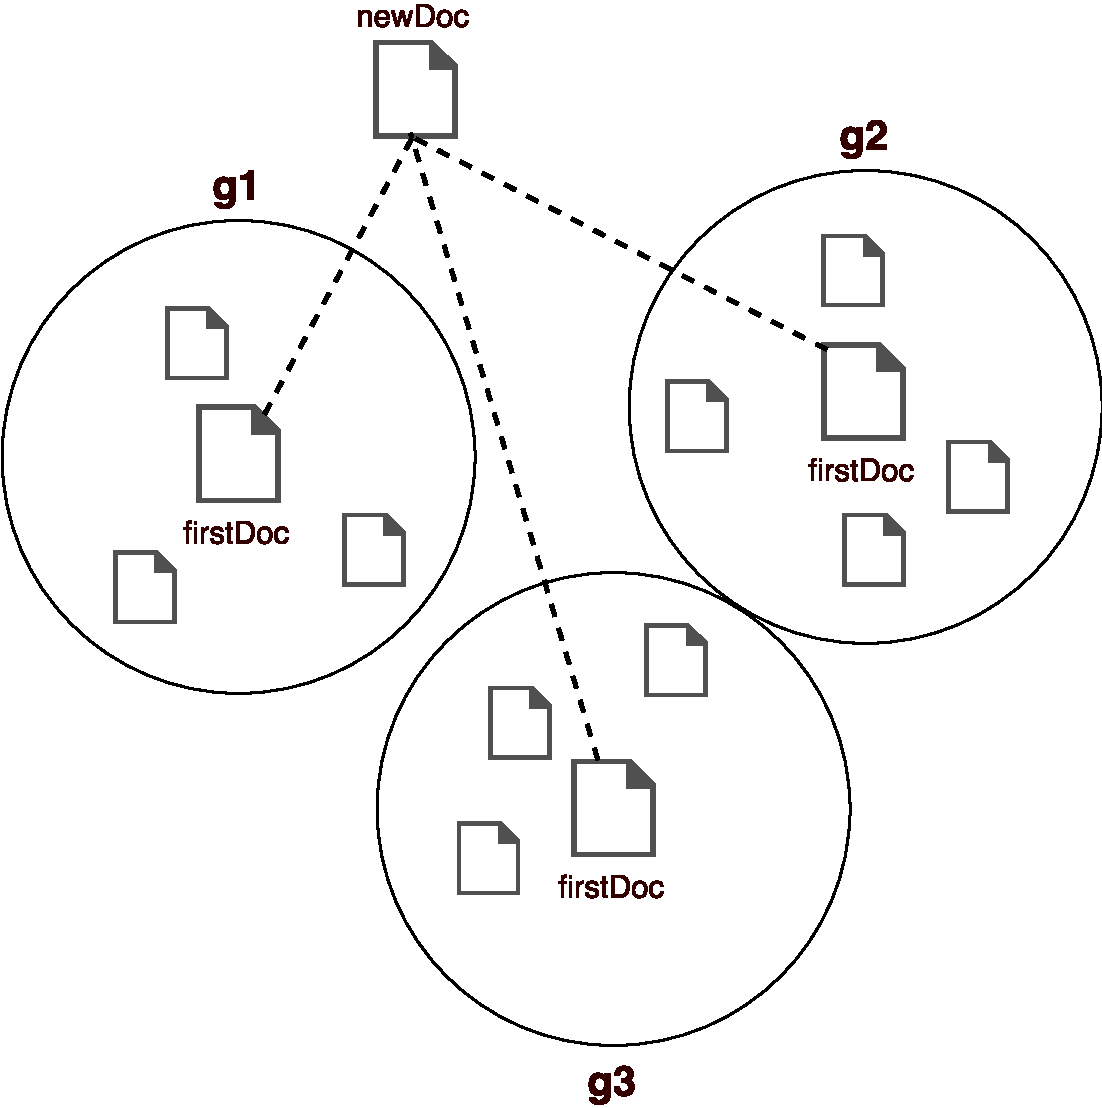
\includegraphics[width=0.65\textwidth]{Clustering_NER2.pdf}
			\caption{...}
		\end{center}
	\end{figure}
	
	\subsubsection{Mã giả}
	\begin{algorithm}[H]
		\caption{First Story Detection sử dụng gom cụm theo nội dung, boost Named Entity}
		\begin{algorithmic}[1]
			\REQUIRE luồng bài viết từ Twitter
			\ENSURE các cụm bài viết ứng với mỗi story phát hiện được, có thứ tự xếp hạng giữa các cụm

			\ForEach{document $d$ trong toàn bộ dữ liệu}
				\State $MaxScore_d \leftarrow 0$
				\State $IDMaxScore_d \leftarrow \emptyset$
				\ForEach{cụm g trong tập hợp cụm G}
%					\State tính $Score_d[g]$: độ tương đồng giữa $d$ với $g.firstDoc$, chỉ dùng một số topTerms của $g$
					\State tính $Score_d[g] \leftarrow similarity(d, g.firstDoc, g.topTerms)$
					
					\IF{$MaxScore_d < Score_d[g]$}
						\State $MaxScore_d \leftarrow Score_d[g]$
						\State $IDMaxScore_d \leftarrow g.groupID$
					\ENDIF
				\ENDFOR
				
				\IF{$MaxScore_d$ > MergeThreshold}
					\State gán $d$ vào cụm $IDMaxScore_d$
				\ELSE
					\State tạo cụm $g_{new}$
					\State $g_{new}.firstDoc \leftarrow d$
				\ENDIF
			\ENDFOR
		\end{algorithmic}
	\end{algorithm}
	Chú thích thuật toán:
	\begin{itemize}
		\item $MaxScore_d$: chứa độ tương đồng lớn nhất giữa document d và các cụm đã có
		\item $IDMaxScore_d$: ID của cụm tương đồng nhất với document d
		\item $Score_d[g]$: độ tương đồng giữa document d với cụm g 
		\item $MergeThreshold$: ngưỡng để xét một document có thuộc về cụm/có là first story hay không
	\end{itemize}
	Độ tương đồng giữa 2 document được tính bằng các công thức sau:
	\begin{equation}
			similarity(d_1, d_2) = \sum_{t \in d_1,\ t \in g.topTerms}[tf(t, d_2) \times idf(t) \times boost(t)]
	\end{equation}
	\begin{equation}
		tf(t, d) = \frac{count(t \ in\ d)}{size(d)}
	\end{equation}
	\begin{equation}
		idf(t) = 1 + \log\frac{N}{count(m\ has\ t)}
	\end{equation}
	Các kí hiệu: 
	\begin{itemize}
		\item $similarity(d_1, d_2)$: độ tương đồng giữa document d1 và document d2
		\item $boost(t)$: giá trị boost cho term t, nếu t là một danh từ riêng (Named Entity) thì boost(t) > 1, ngược lại boost(t) = 1
		\item $count(t \in d)$: tần suất term t xuất hiện trong trong document d
		\item $size(d)$: số lượng term của document d
		\item $tf(t, d)$: tần suất xuất hiện (theo phần trăm) của term t trong document d
		\item $idf(t)$: giá trị inverse document frequency của term t
	\end{itemize}
	
	Ưu điểm:
	\begin{itemize}
		\item 
	\end{itemize}
	Nhược điểm:
	\begin{itemize}
		\item 
	\end{itemize}
	
%========================================================================================================================

\subsection{Thuật toán Locality Sensitive Hashing}
	\subsubsection{Ý tưởng}
	Thuật toán tìm kiếm láng giềng gần nhất tốn rất nhiều chi phí khi lượng dữ càng lớn (O(nd) với n là số lượng document hiện có và d là số chiều của mỗi document). Thay vào đó, ta có thể giải bài toán tìm \textit{xấp xỉ} láng giềng gần nhất. Một thuật toán để giải quyết bài toán này là \textit{Locality Sensitive Hashing (LSH)}. <cần cite Indyk \& Motwani (1998)??>
	
	LSH hoạt động bằng cách chia không gian biểu diễn dữ liệu thành nhiều vùng riêng biệt bằng một tập các siêu phẳng ngẫu nhiên. Khi tìm láng giềng cho một document, ta chỉ cần so sánh nó với các document thuộc chung vùng không gian, nhờ đó giảm đáng kể chi phí tính toán. Ta có thể xem mỗi cách chia không gian này ứng với một hash table, và số bit của hash code bằng với số lượng siêu phẳng đã dùng để chia không gian.
	
	Vì các siêu phẳng được chọn một cách ngẫu nhiên, nên đôi khi các document gần nhau có thể bị phân vào vùng khác nhau. Do đó ta thường dùng nhiều hash table để tăng thêm khả năng tìm được láng giềng gần nhất.	
%	LSH sử dụng một họ hash function (hàm băm) có đặc điểm: những documents càng tương đồng với nhau thì càng có khả năng trùng hash code (mã băm) với nhau. Mỗi document mới sẽ được đưa qua hash function tính toán, và sau đó được so sánh với các document có cùng hash code với nó.\\
%	Ta có thể hình dung phương pháp của LSH như sau: Trong không gian biểu diễn dữ liệu $k$ chiều, mỗi bit trong hash code ứng với một siêu phẳng phân không gian thành 2 vùng... (giải thích lại)
	
	\subsubsection{Minh họa cách tính hash code cho LSH}
	Xét trường hợp một document $d$ biểu diễn dưới dạng vector $d = (0,1,0,1,1,1,0)$, và ta chọn sử dụng hash code có 4 bit (dùng 4 siêu phẳng để chia không gian dữ liệu).\\
	Mỗi hash table được khởi tạo bằng cách: tạo 4 vector ngẫu nhiên ứng với 4 siêu phẳng, số chiều bằng với số chiều vector $d$
	Cách tính hash code của document $d$ trong một hash table như sau: lần lượt tính tích vô hướng của vector $d$ với từng vector của siêu phẳng, nếu tích dương thì bit đó có giá trị 1, nếu tích âm thì có giá trị 0. 
	
	\begin{figure}[ht]
		\begin{center}
			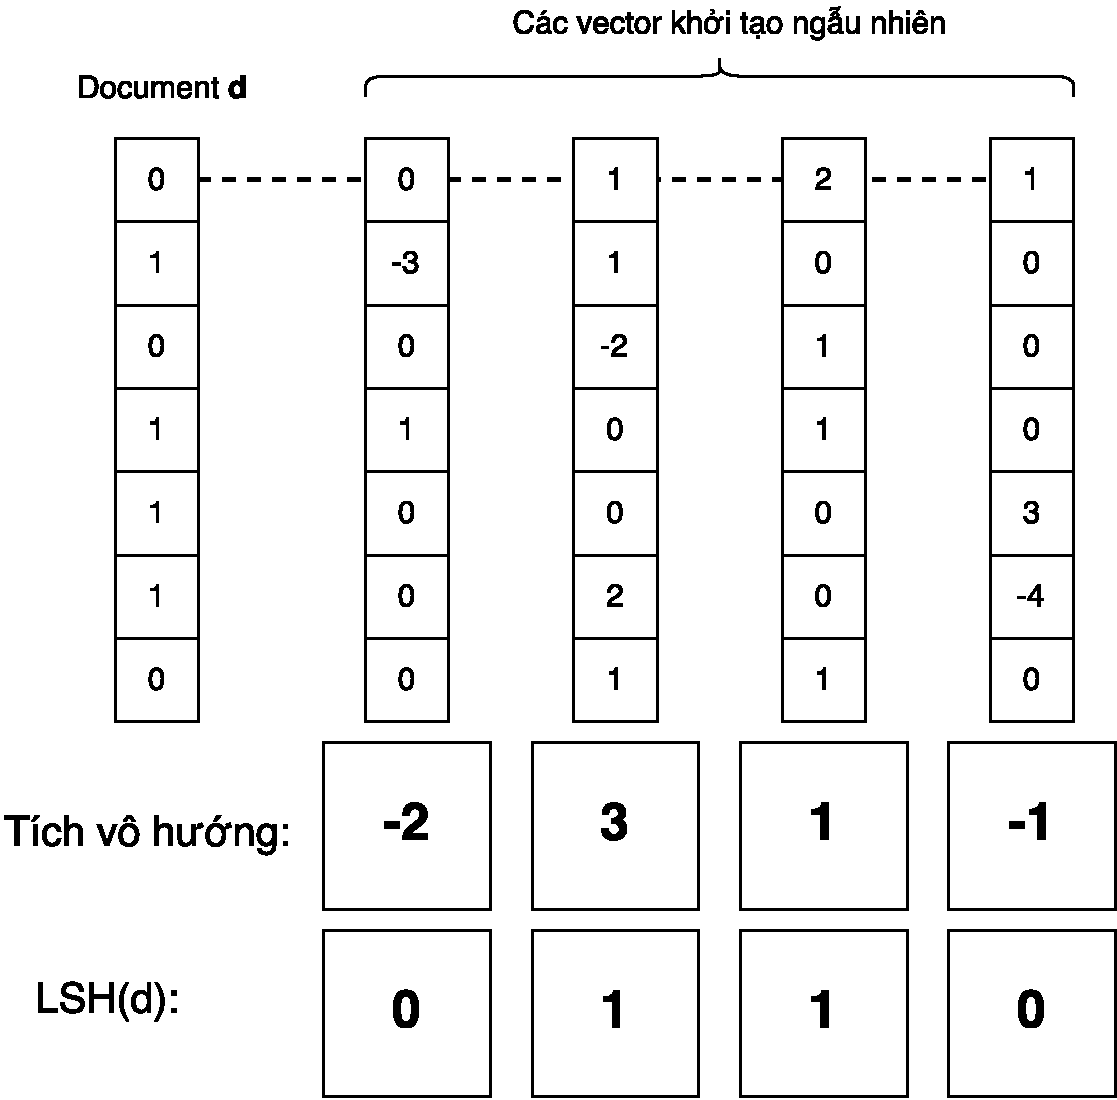
\includegraphics[width=0.65\textwidth]{LSH.pdf}
			\caption{Cách tính hash code cho một document trong một hash table}
		\end{center}
	\end{figure}
	
	
	\subsubsection{Mã giả}
	\begin{algorithm}[H]
		\caption{Locality Sensitive Hashing}
		\begin{algorithmic}[1]
			\REQUIRE luồng bài viết từ Twitter, giá trị ngưỡng t
			\ENSURE những document được cho là first story
			\State Khởi tạo L hash tables
			\ForEach{document $d$ mới}
				\ForEach{hash table $l$ trong $L$}
					\State Tính hash code cho document d: $LSH_l(d)$
					\State Thêm tất cả các documents d' có $LSH_l(d') = LSH_l(d)$ vào tập $S$
				\ENDFOR
				\State $dis_{min}(d) = 1$
				\ForEach{document $d'$ trong $S$}
					\IF {$distance(d,d') < dis_{min}(d)$}
					\STATE $dis_{min}(d) = distance(d,d')$
		 			\ENDIF
				\ENDFOR
				\IF{$dis_{min}(d) >= t$}
					\STATE d là một first story
				\ENDIF
			\ENDFOR
			
		\end{algorithmic}
	\end{algorithm}
	Chú thích thuật toán:
	\begin{itemize}
		\item $t$: ngưỡng để xét một document có phải là first story hay không
		\item $LSH_l(d)$: hash code của document $d$ trong hash table thứ $l$
		\item $dis_{min}(d)$: khoảng cách giữa document $d$ với document gần nhất
		
	\end{itemize}
	
	Ưu điểm:
	\begin{itemize}
		\item Chi phí tính toán thấp do không cần so sánh toàn bộ các document với nhau.
		\item Độ chính xác tương đối tốt
	\end{itemize}
	Nhược điểm:
	\begin{itemize}
		\item Cần tìm chọn các thông số như: số lượng hash table, số lượng bit trong hash code,... tốt để cho kết quả chính xác.
		\item Có thể không tìm được document thật sự tương đồng nhất, trong trường hợp các điểm không được chia vào cùng vùng trong không gian do cách thiết lập của các hash tables/functions.
	\end{itemize}
	
	\begin{algorithm}[H]
		\caption{Locality Sensitive Hashing kết hợp với **************************}
		\begin{algorithmic}[1]
			\boldmath
			\REQUIRE luồng bài viết từ Twitter, giá trị ngưỡng t
			\ENSURE những document được cho là first story
			\State Khởi tạo L hash tables
			\ForEach{document $d$ mới}
				\ForEach{hash table $l$ trong $L$}
					\State Tính hash code cho document d: $LSH_l(d)$
					\State Thêm tất cả các documents d' có $LSH_l(d') = LSH_l(d)$ vào tập $S$
				\ENDFOR
				\State $dis_{min}(d) = 1$
				\ForEach{document $d'$ trong $S$}
					\unboldmath
					\IF {$distance(d,d') < dis_{min}(d)$}
					\State $dis_{min}(d) = distance(d,d')$
					\ENDIF
				\ENDFOR
				\IF{$dis_{min}(d) >= t$}
					\State Tính khoảng cách giữa d với một lượng (1000-3000) documents mới nhất trong bộ dữ liệu, cập nhật $dis_{min}(d)$ nếu có thay đổi.
				\ENDIF
				\IF{$dis_{min}(d) >= t$}
					\STATE d là một first story
				\ENDIF
			\ENDFOR		
			
		\end{algorithmic}
	\end{algorithm}
	
\section{Tiếp cận bằng phương pháp phân lớp}